\documentclass{article}

\usepackage{graphicx}
\usepackage{tikz}
\usepackage{tikzsymbols}
\usetikzlibrary{calc,patterns,shapes.geometric}
\pagestyle{empty}
\usepackage[margin=0pt]{geometry}
\geometry{papersize={14in,12in}}

\def\centerarc[#1](#2)(#3:#4:#5){\draw[#1] ($(#2)+({#5*cos(#3)},{#5*sin(#3)})$) arc (#3:#4:#5);}

\begin{document}
	\begin{figure}
		\centering
		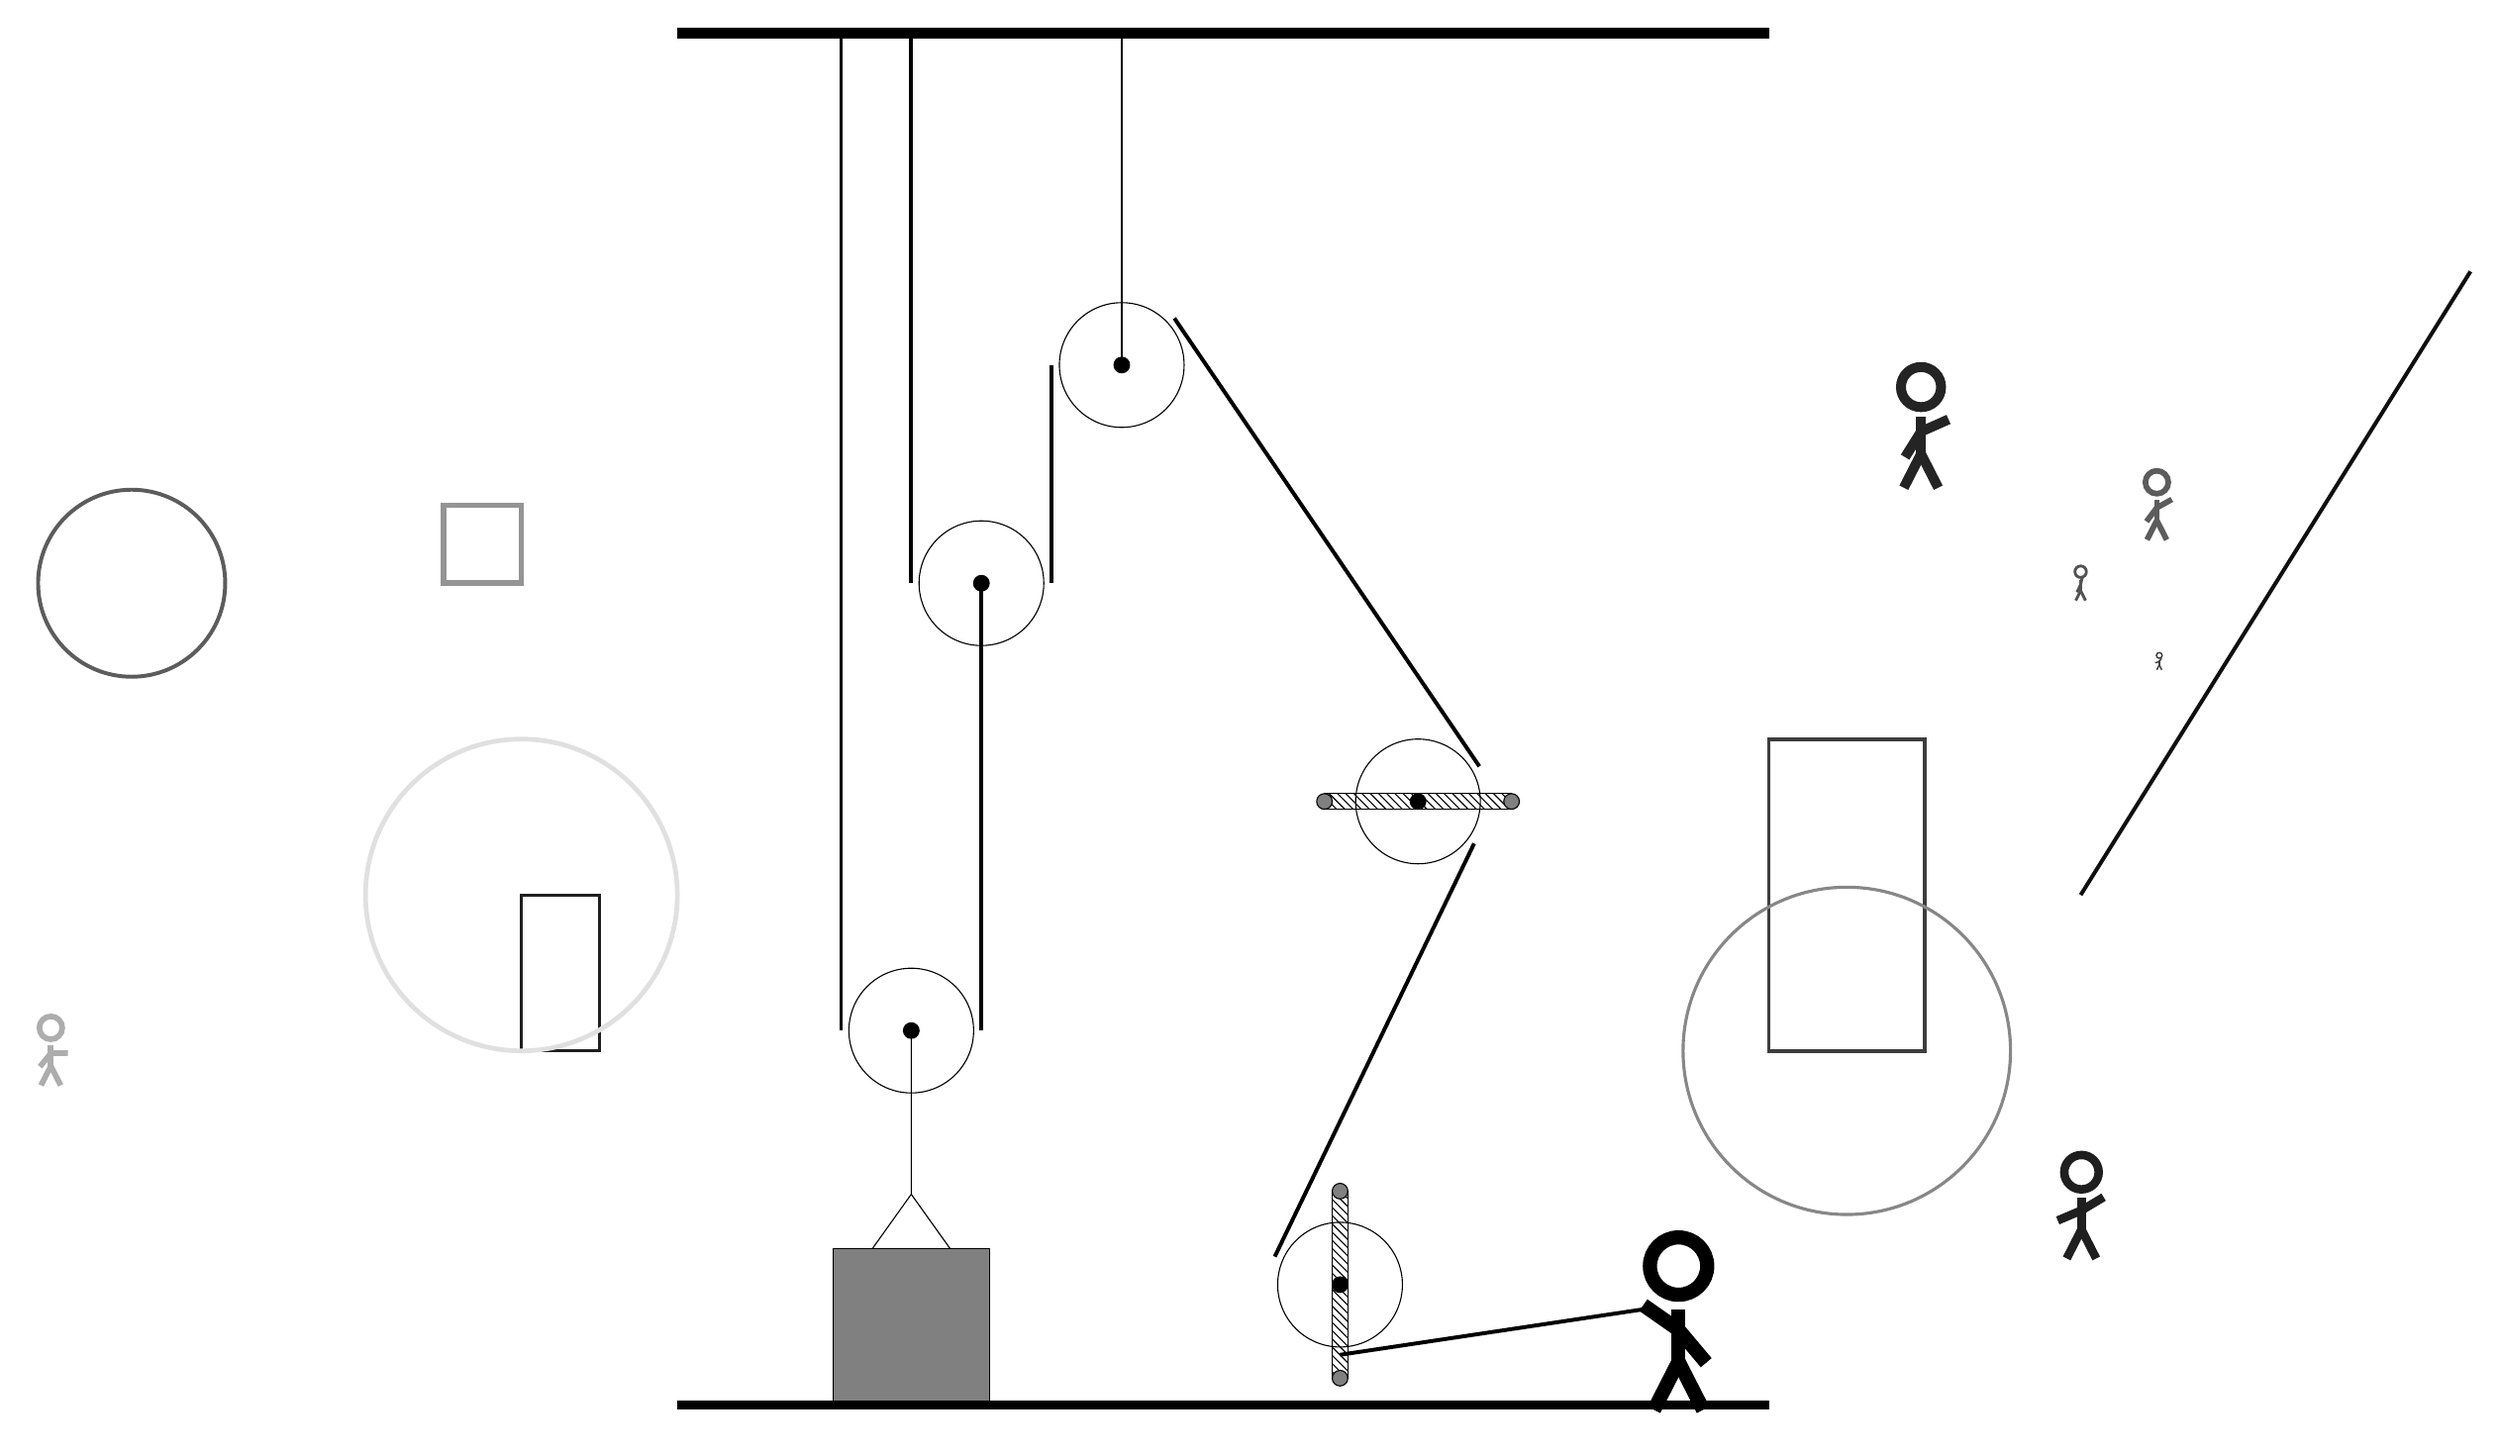
\begin{tikzpicture}
			%%%%% START %%%%%
			
			\draw[fill=black] (-2, 14) rectangle (12, 14.125);
			
			\draw (1, 1.26) circle (0.8);
			\draw[fill=black] (1, 1.26) circle (0.1);
			
			\draw (1.9, 7.0) circle (0.8);
			\draw[fill=black] (1.9, 7.0) circle (0.1);
			
			\draw [line width=0.5mm, color=black!64](-9, 7) circle (1.2);
			
			\draw[line width=0.5mm, color=black!94](16, 3) -- (21, 11);
			\draw[line width=0.4mm, color=black!88] (-3, 1) rectangle (-4, 3);
			\node[line width=0.2mm, color=black!32] at (-10, 1) {\Strichmaxerl[4][51][1]};
			
			\node[line width=0.6mm, color=black!64] at (17, 8) {\Strichmaxerl[4][53][29]};
			
			\node[line width=0.3mm, color=black!86] at (14, 9) {\Strichmaxerl[7][58][24]};
			\draw[line width=0.7mm, color=black!42] (-4, 8) rectangle (-5, 7);
			\draw[line width=0.5mm, color=black!76] (12, 1) rectangle (14, 5);
			\draw [line width=0.4mm, color=black!47](13, 1) circle (2.1);
			\draw [line width=0.6mm, color=black!12](-4, 3) circle (2.0);
			\node[line width=0.3mm, color=black!68] at (16, 7) {\Strichmaxerl[2][65][77]};
			
			\node[line width=0.7mm, color=black!88] at (16, -1) {\Strichmaxerl[6][23][31]};
			\node[line width=0.2mm, color=black!75] at (17, 6) {\Strichmaxerl[1][13][59]};
			
			\draw (3.7, 9.8) circle (0.8);
			\draw[fill=black] (3.7, 9.8) circle (0.1);
			\draw[thick] (3.7, 9.8) -- (3.7, 14);
			
			\draw (6.5, -2) circle (0.8);
			\draw[fill=black] (6.5, -2) circle (0.1);
			\draw[pattern=north west lines, pattern color=black] (6.4, -0.8) rectangle (6.6, -3.2);
			\draw[fill=black!50] (6.5, -0.8) circle (0.1);
			\draw[fill=black!50] (6.5, -3.2) circle (0.1);
			
			\draw (7.5, 4.2) circle (0.8);
			\draw[fill=black] (7.5, 4.2) circle (0.1);
			\draw[pattern=north west lines, pattern color=black] (6.3, 4.3) rectangle (8.7, 4.1);
			\draw[fill=black!50] (6.3, 4.2) circle (0.1);
			\draw[fill=black!50] (8.7, 4.2) circle (0.1);
			
			\draw (1, 1.26) -- (1, -0.84) -- (0.5, -1.54) -- (1.5, -1.54) -- (1, -0.84);
			\draw[fill=black!50] (0, -1.54) rectangle (2, -3.54);
			
			\draw[line width=0.5mm] (0.1, 14) -- (0.1, 1.26);
			\centerarc[line width=0.5mm](1, 1.26)(180:360:0.9);
			\draw[line width=0.5mm](1.9, 1.26) -- (1.9, 7.0);
			\draw[line width=0.5mm] (1.0, 14) -- (1.0, 7.0);
			\centerarc[line width=0.5mm](1.9, 7.0)(180:360:0.9);
			\draw[line width=0.5mm](2.8, 7.0) -- (2.8, 9.8);
			\centerarc[line width=0.5mm](3.7, 9.8)(35:180:0.9);
			\draw[line width=0.5mm] (4.375, 10.4) -- (8.2875, 4.65);
			\centerarc[line width=0.5mm](7.5, 4.2)(215:135:-0.9);
			\draw[line width=0.5mm](8.22, 3.66) -- (5.663, -1.64);
			\centerarc[line width=0.5mm](6.5, -2)(-30:100:-0.9);
			\draw[line width=0.5mm](6.5, -2.9) -- (10.5, -2.3);
			
			\node at (10.8, -2.5) {\Strichmaxerl[10][-35][-50]};
			
			\draw[fill=black] (-2, -3.5) rectangle (12, -3.6);
			
			%%%%% END %%%%%
		\end{tikzpicture}
	\end{figure}	
\end{document}